\documentclass[12pt]{scrartcl}

\usepackage[utf8]{inputenc}
\usepackage[naustrian]{babel}
\usepackage{caption}
\usepackage{graphicx}
\usepackage{verbatim}
\usepackage[T1]{fontenc}
\usepackage{lmodern}
\usepackage{subcaption}
\usepackage{amsfonts}
\usepackage{listings}
\usepackage{float}

%pdfs
\usepackage{pdfpages}
\usepackage{tikz}

%page borders
\usepackage{geometry}
\geometry{left=2.5cm,right=2.5cm,top=3cm,bottom=2.5cm}

\usepackage{minted}
\setminted {
	%style=igor, %borland, autumn, vs
	encoding=utf-8,
	autogobble,
	tabsize=4,
	linenos,
	breaklines,
	keywordcase=upper,
	%escapeinside=||
	%bgcolor=bg
	%frame=single
}

\newenvironment{code}{\captionsetup{type=listing}}{}

%title/footer/header values
\usepackage{titling}
\title{DES3UE Übung 4}
\author{Elias Leonhardsberger}
\date{\today{}, Hagenberg}

%footer/header
%\usepackage[automark]{scrpage2}
%\pagestyle{headings}
%\clearscrheadfoot
%\ihead{\thetitle}
%\chead{\theauthor}
%\ohead{\today}
%\cfoot{Seite \pagemark}

\begin{document}
\clearpage
\thispagestyle{empty}
\begin{tikzpicture}[remember picture, overlay]
	\node at (current page.center) {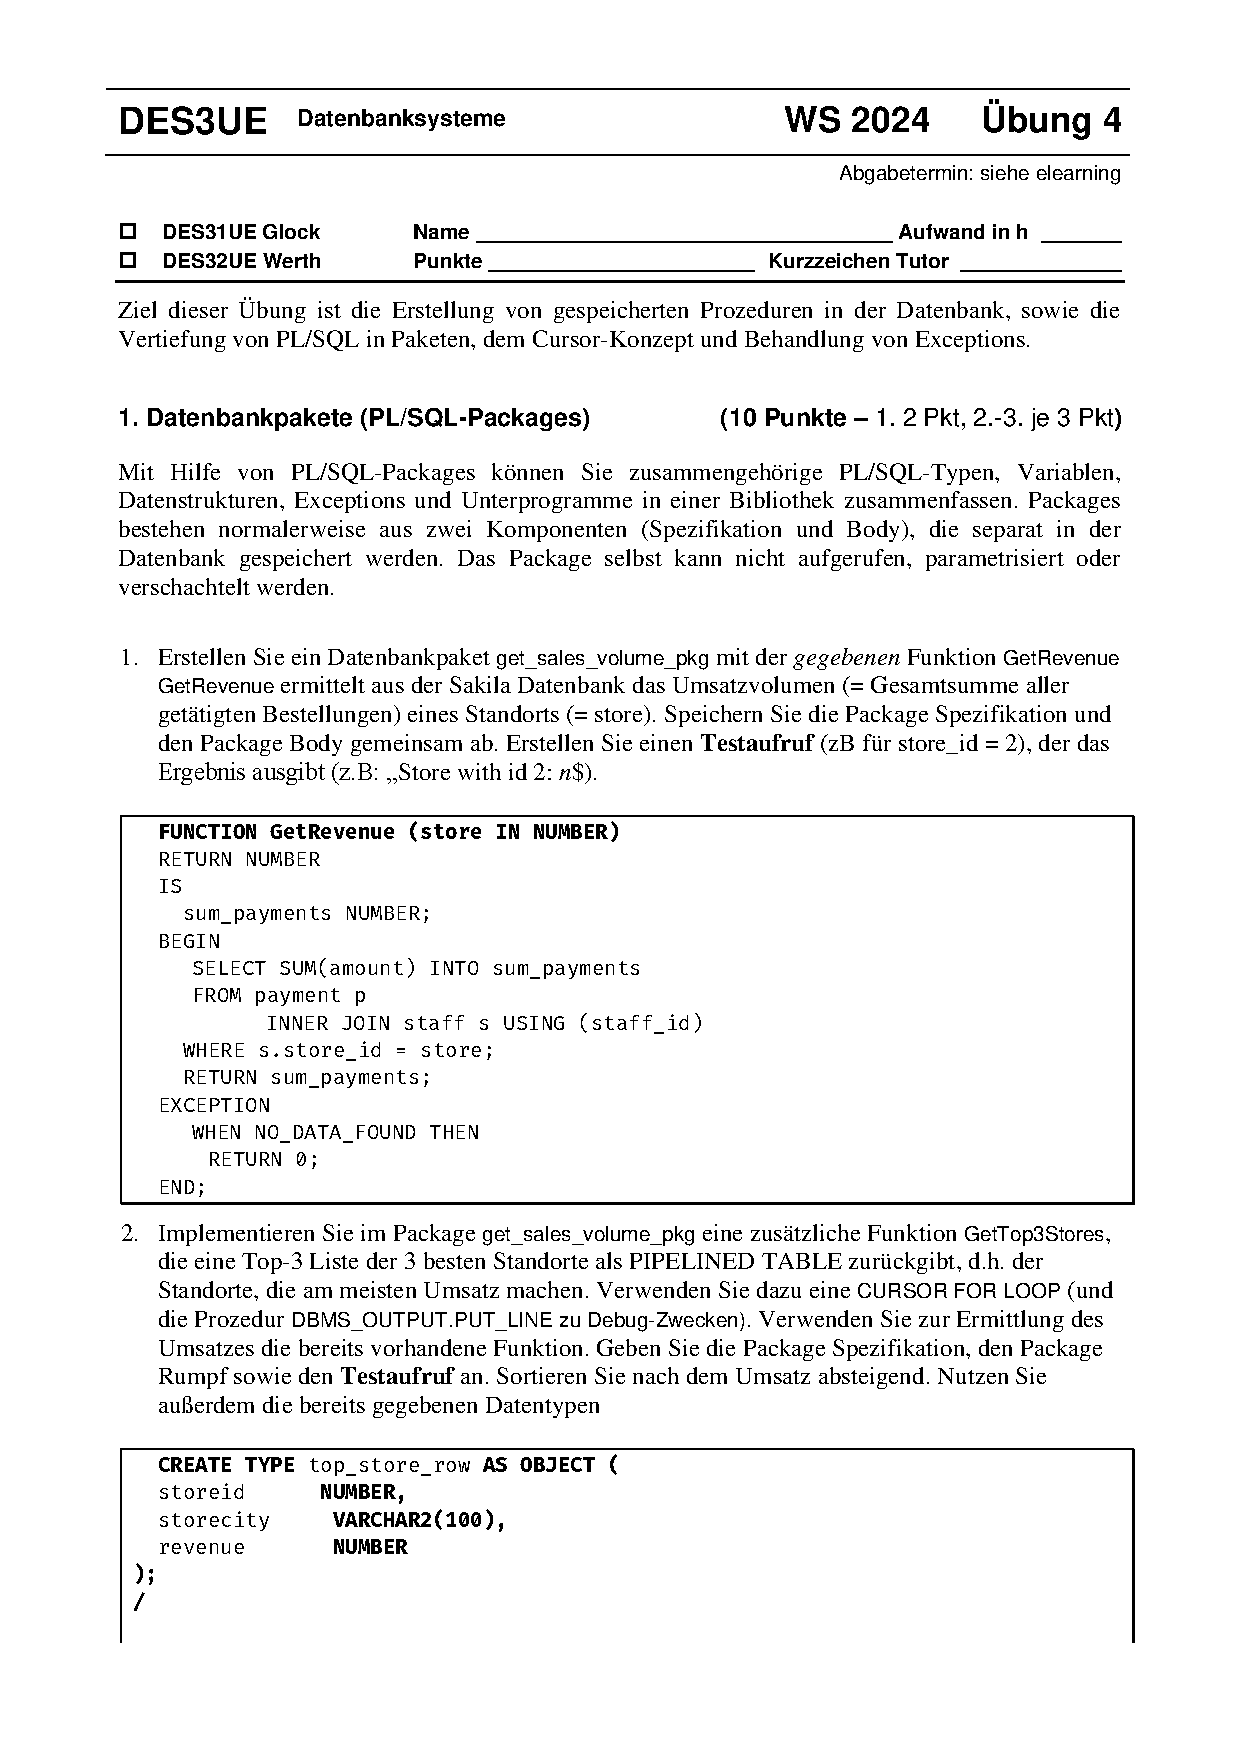
\includegraphics[page=1]{Angabe.pdf}};
	\begin{scope}[shift={(current page.south west)},every node/.style={anchor=base west}]
		\node at (8.5cm, 26.4cm) {\theauthor};
		\node at (17.2cm, 26.4cm) {3};
		\node at (1.87cm, 26.35cm) {X};
	\end{scope}
\end{tikzpicture}

\includepdf[pages=2-3]{Angabe.pdf}

\maketitle
\tableofcontents

\pagebreak

\section{Datenbankpakete (PL/SQL-Packages)}

\subsection{SQL}
\inputminted{sql}{../ue4_1.sql}

\subsection{Ergebnisse}
\begin{figure}[h]
	\centering
	
\includegraphics[width=0.8\textwidth]{../ue4_1_1.png}
	\caption{Ergebnis Aufgabe 1.1}
\end{figure}

\begin{figure}[h]
	\centering
	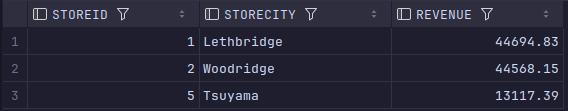
\includegraphics[width=0.8\textwidth]{../ue4_1_2.png}
	\caption{Ergebnis Aufgabe 1.2}
\end{figure}

\begin{figure}[h]
	\centering
	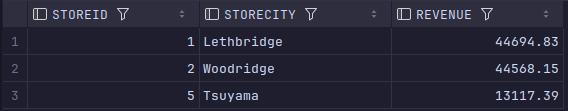
\includegraphics[width=0.8\textwidth]{../ue4_1_3.png}
	\caption{Ergebnis 1 Aufgabe 1.3}
\end{figure}

\begin{figure}[h]
	\centering
	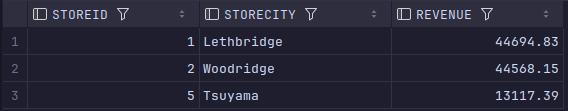
\includegraphics[width=0.8\textwidth]{../ue4_1_3.png}
	\caption{Ergebnis 2 Aufgabe 1.3}
\end{figure}

\section{PL/SQL Prozeduren}

\subsection{SQL}
\inputminted{sql}{../ue4_2.sql}

\subsection{Ergebnisse}
\begin{figure}[h]
	\centering
	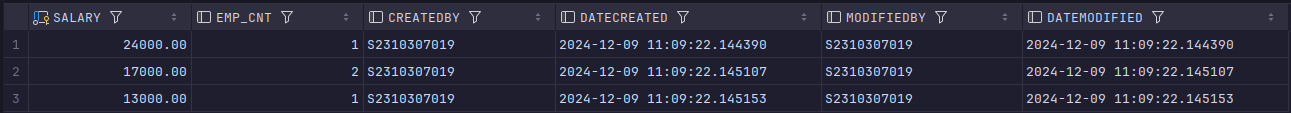
\includegraphics[width=1\textwidth]{../ue4_2.png}
	\caption{Ergebnis Aufgabe 2}
\end{figure}

\section{Cursor mit FOR-UPDATE}

\subsection{SQL}
\inputminted{sql}{../ue4_3.sql}

\subsection{Ergebnisse}
\begin{figure}[h]
	\centering
	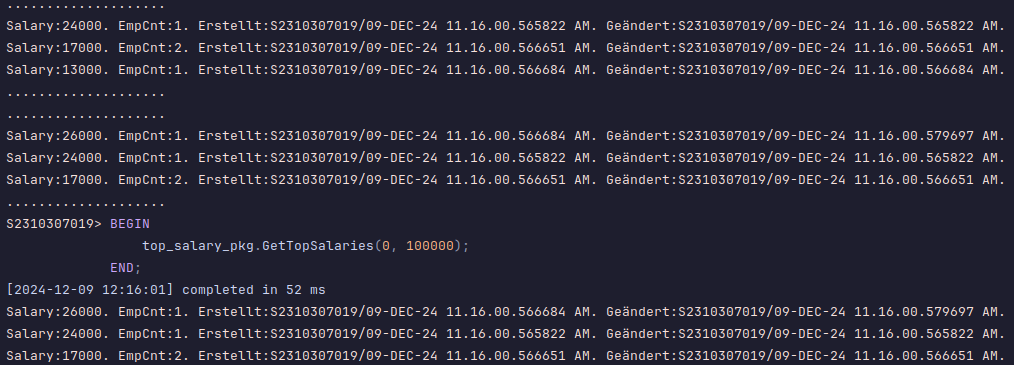
\includegraphics[width=0.8\textwidth]{../ue4_3_1.png}
	\caption{Ergebnis Aufgabe 3.1-3.2}
\end{figure}

\end{document}